\documentclass[12pt]{article}
\usepackage{amsmath}

\usepackage{graphicx}
\graphicspath{ {/home/user/COEP/Sem 3/DTL} }

\usepackage{caption}
\usepackage{subcaption}

\usepackage{csvsimple}

\title{\textbf{College Of Engineering Pune\\Department Of Applied Mathematics\\MA19001 : Univerate Calculus\\ End Semester Examination.}}
\date{}
\begin{document}
\maketitle

Date: \date{{22/11/2022}
\\\hspace*{0.6cm}Program : FY B.Tech Sem II
\\\hspace*{0.6cm}Duration : 2 hours
\\\hspace*{0.6cm}Maximum Marks : 40
\\\\\textit{\textbf{Instructions : }\\1.Write your MIS Number on Question Paper and Answer Sheet.\\2.Do not write anything else on the Question paper.\\3.Mobile phones, digital watches or any other electronic gadgets are strictly prohibited.\\4.Programmable calculators are not permitted.\\5.Exchange of any material during the examination is not allowed.}

\tableofcontents
\newpage
\begin{center}
\section{\textbf{Maths Paper}}
\subsection{\textbf{Section - A\hspace*{2cm}[20 Marks]}}

\end{center}
(Q1)  Identify the largest possible domain of the following functions. Also find the extreme values of the functions and the points where they occur.
\\\hspace*{12cm}[5 Marks]
\\$(a)f(x) = x^2 + 8x + 9 $\\
$(b)f(x) = x^{3} +{2x} + 4 $ \\
$(c)f(x) = \sqrt{x^2-1}$\\\\\\

(Q2) Let $f(x) = |x^{3}-9x|$. 
\\Does f'(x) exist when $x = 0,3$? Find all the critical points of f(x) and hence determine all extrema of the given function.\hspace*{4cm}[3 Marks]\\\\\\

(Q3)  Say True/ False. Justify your answer.\hspace*{4cm}[4 Marks]
\\(a) If a function has global maximum then it has local maximum.
\\(b) If a function is continuous then it has global minimum.
\\(c) If a function is defined on a closed interval then it has global extrema.
\\(d) If a function is such that its derivative is not zero at any point then it has no global extrema.\\\\\\

(Q4) Find a value of c that makes the function \hspace*{3cm}[2 Marks]\\
\begin{math}
  f(x)=\left\{
    \begin{array}{ll}
      c ,  & \mbox{if $x=0$}.\\
      \frac{9x - \sin 3x}{x^3}, & \mbox{otherwise}.
    \end{array}
  \right.
\end{math}\\\\\\

(Q5) A window is to be made in the form of a rectangle surmounted by a semicircular portion with diameter equal to the base of the rectangle. The rectangular portion is to be of clear glass and the semicircular portion is to be of coloured glass admitting only half as much light per square foot as the clear glass. If the total perimeter of the window is to be p feet, find the dimensions of the window which will admit the maximum light.
\\( width=$ \frac{4p} {3\pi +8} and height = \frac{p(\pi +4)}{3\pi +8}$. )\hspace*{6.1cm}[2 Marks]\\\\\\

(Q6)Prove the following inequalities.\hspace*{5cm}[4 Marks]
\\(a)$|tan ^{-1}- \tan ^{-1}y|<|x-y|$ for all x and y in R.
\\(b)$\frac{b-a}{\sqrt{1-a^2}}< \sin ^{-1}b -\sin ^{-1}a <\frac{b-a}{\sqrt{1-b^2}} $ \\ \hspace*{0.6cm} for $0<a<1$  and  $<b<1$

\newpage
\begin{center}
\subsection{\textbf{Section - B\hspace*{2cm}[20 Marks]}}
\end{center}

(Q1) Prove that the following sequences are convergent by showing that they are monotone and bounded. Also find their limits.\hspace*{1.5cm}[4 Marks]\\
(a)$a_{1}=2,a_{n+1} = \frac{1}{2}(a_{n} + \frac{2}{a_{n}}),$ for all $n>1$ \\
(b)$a_{1}=\sqrt{2} ,a_{n+1}=\sqrt{2+a_{n}}$ for all $n>1$  \\
(c)$a_{1}=1 ,a_{n+1}=a_{n} + \frac{1}{2^{n}}$ for all $n>1$\\\\\\

(Q2) Find the volumes of the solids generated by revolving the regions bounded by the lines and curves about the y- axis.\hspace*{3cm}[4 Marks]\\
(a) The region enclosed by $x = \sqrt{5}y^2 , x = 0, y=1,y= -1$\\
(b) The region enclosed by $x = y^\frac{3}{2} , x=0 , y= 2$\\
(c) The region enclosed by $ x = \sqrt{2\sin 2y}, 0 \leq y \leq \pi/2 , x=0.$\\\\\\

(Q3)Find the Fourier series expansions of the following periodic functions for the given period.\hspace*{9cm}[4 Marks]\\
(a) $f(x) = |\sin x| ({-\pi}< x < \pi)$\\
(b)$ f(x) = x^3 ({-1} < x < 1)$\\
(c)f(x) = \begin{math}
  \left\{
    \begin{array}{ll}
     $ 4+x $,  & \mbox{if $-4<x<0$}.\\
      $4-x$, & \mbox{if $0<x<4$}.
    \end{array}
  \right.
\end{math} 
\\(d) f(x) =  \begin{math}
  \left\{
    \begin{array}{ll}
     x^{2},  & \mbox{if ${-\frac{\pi}{2}}<x<\frac{\pi}{2}$}.\\
      $4-x$, & \mbox{if $\frac{\pi}{2}<x<\frac{3\pi}{2}$}.
    \end{array}
  \right.
\end{math} 
\\(e)f(x) = $e^{ax} (0<x<2{\pi})$\\\\\\

(Q4)Solve the following : \hspace*{7cm}[4 Marks]
\\(a)Prove the trigonometric identity $\sin 2x = 2 \sin x \cos x$ using Fourier series expansion.
\\(b)Find the Fourier series of the periodic function that is obtained by passing the voltage $v(t) = V_0 \cos(100\pi t)$ through a half-wave rectifier.\\\\\\

(Q5) If 
$A =
\begin{bmatrix}
1 & 2 & 3\\
4 & 5 & 6\\
7 & 8 & 9\\
\end{bmatrix}
$ , find $A^{-1}$. \hspace*{4cm}[4 Marks]

\newpage
\begin{center}
\section{\textbf{Table}}
\end{center}

\begin{table}[h]
\begin{center}
\caption{Stock Market Chart - Current Analysis of Stocks}
\label{tab:table1}

\begin{tabular}{1|1|1|1|}
\hline
\textbf{Company} & \textbf{High} & \textbf{Low} & \textbf{Val.(cr.)}\\\hline
\textbf{Infosys} & 1588.00 & 1562.00 & 535.74\\ \hline
\textbf{ONGC} & 135.90 & 132.90 & 150.59\\ \hline
\textbf{Infosys} & 19,849.30 & 19,550.05 & 93.06\\ \hline

\end{tubular}
\end{center}
\end{table}

\begin{filecontents*}{grade.csv}
name,givenname,matriculation,gender,grade
Maier,Hans,12345,m,1.0
Huber,Anna,23456,f,2.3
Weisbaeck,Werner,34567,m,5.0
\end{filecontents*}

\begin{table}[h]
\begin{center}
\caption{Name and Matr no. from CSV file}
\label{tab:table2}

\begin{tabular}{l|c}
\bfseries Person & \bfseries Matr.~No.
\csvreader[head to column names]{grade.csv}{}
{\\\hline\givenname\ \name & \matriculation}

\end{tabular}
\end{center}
\end{table}

\newpage
\begin{center}
\section{\textbf{Images}}
\end{center}

The universe is immense and it seems to be homogeneous, 
in a large scale, everywhere we look at.\\

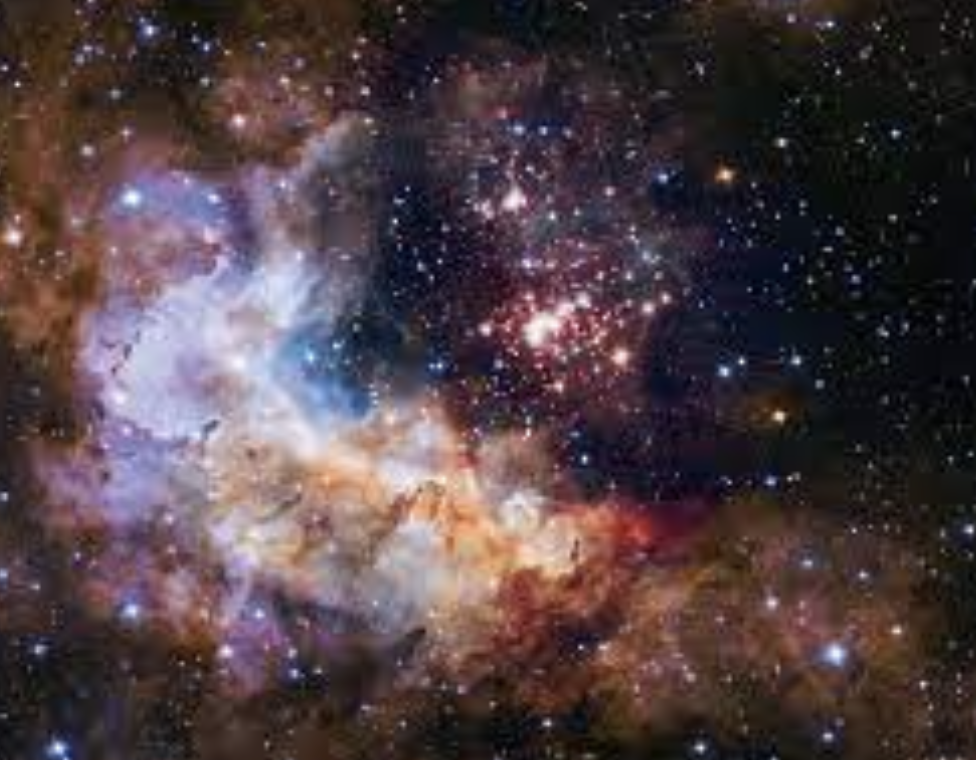
\includegraphics[width=8cm, height=8cm]{universe}\\

There's a picture of a galaxy above

\newpage
\begin{center}
\section{\textbf{Bibliography}}
\end{center}
\section*{Black Holes}
A black hole is a region of spacetime where gravity is so strong that nothing, including light or other electromagnetic waves, has enough energy to escape it ~\cite{1}.The theory of general relativity predicts that a sufficiently compact mass can deform spacetime to form a black hole.~\cite{2, 3} The boundary of no escape is called the event horizon. Although it has a great effect on the fate and circumstances of an object crossing it, it has no locally detectable features according to general relativity.~\cite{4} In many ways, a black hole acts like an ideal black body, as it reflects no light.~\cite{5, 6} Moreover, quantum field theory in curved spacetime predicts that event horizons emit Hawking radiation, with the same spectrum as a black body of a temperature inversely proportional to its mass. This temperature is of the order of billionths of a kelvin for stellar black holes, making it essentially impossible to observe directly.
\section*{Bibliography}
\begin{thebibliography} {}
\bibitem {1} Wald 1984, pp. 299–300
\bibitem {2} Wald, R. M. (1997). "Gravitational Collapse and Cosmic Censorship". In Iyer, B. R.; Bhawal, B. (eds.). Black Holes, Gravitational Radiation and the Universe. Dordrecht: Springer. pp. 69–86. arXiv:gr-qc/9710068. doi:10.1007/978-94-017-0934-7. ISBN 978-9401709347.
\bibitem {3} Overbye, Dennis (8 June 2015). "Black Hole Hunters". NASA. Archived from the original on 9 June 2015. Retrieved 8 June 2015.
\bibitem {4} Hamilton, A. "Journey into a Schwarzschild black hole". jila.colorado.edu. Archived from the original on 3 September 2019. Retrieved 28 June 2020.
\bibitem {5} Schutz, Bernard F. (2003). Gravity from the ground up.
\bibitem {6} Davies, P. C. W. (1978). "Thermodynamics of Black Holes".

\end{thebibliography}

\end{document}